\chapter{Background}
\label{ch.fundamentation}

	This chapter presents the theoretical background of multiple processor
	systems from a hardware and software perspective.
	Specifically, Section \ref{sec.multiprocessors} and Section \ref{sec.multicomputers}
	will address details about multiprocessors and multicomputers, respectively.
	Subsequently, Section \ref{sec.mppa} will present the \mppa processor.
	Next, Section \ref{sec.hal} will show an overview of the HAL.
	So finally, Section \ref{sec.inter-cluster-communication} will cover the abstraction
	concepts in the Inter-Cluster Communication Module.

% \section{Computer System Organization}
% \section{\OS}

\section{Multiple Processor Systems}
\label{sec.multiple-processor-systems}

	According to Tanenbaum~\cite{tanenbaum:4ed}, exists three models of modern
	multiple processor architectures.
	A shared-memory multiprocessor, a message-passing multicomputer, and a wide
	area distributed systems.
	The sections below address the two first models presenting significant
	hardware and software concepts for the present monograph.

	\subsection{Multiprocessors}
	\label{sec.multiprocessors}

		\begin{figure}[h]
			\centering
			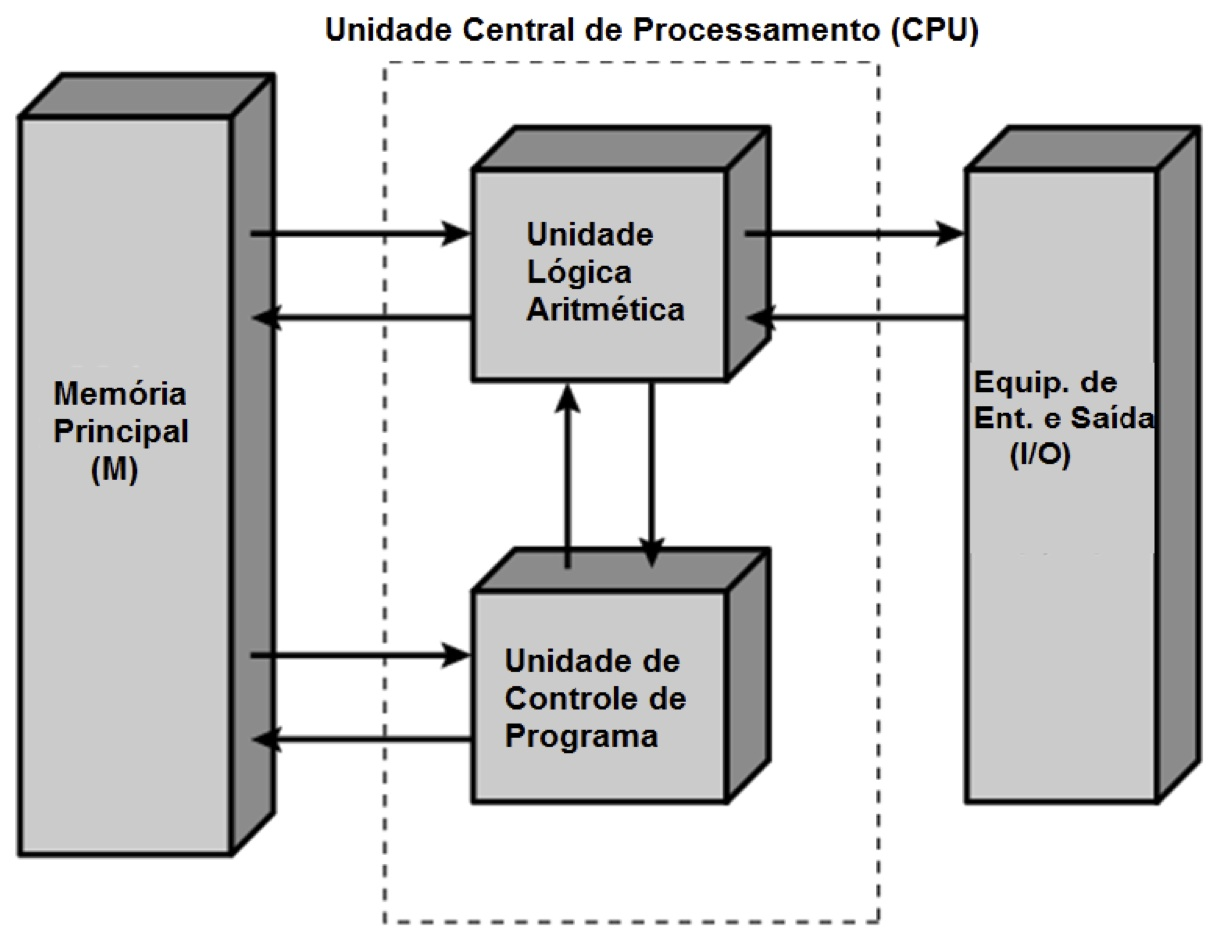
\includegraphics[width=.6\textwidth]{images/neumann.jpg}

			\caption{
				Von Neumann Architecture Model.
			}\par
			\label{fig.neumann}
		\end{figure}

		In the early days of electronic digital computing, John Von Neumann
		proposed an architectural model for computers to be easily programmable~\cite{von-neumann:model}.
		As illustrated in Figure \ref{fig.neumann}, this model describes a \cpu,
		also called core, that loads instructions and data from a Memory Unit,
		dealing with inputs and generating outputs from/to I/O Devices.
		Modern processors still follow this model, but some components and
		behaviors are specialized or replicated to increase performance.

		In this context, a shared-memory multiprocessor is a computer system
		in which two or more \cpus share full access to a common \ram~\cite{tanenbaum:4ed}.
		Concurrency issues begin to appear where are many \cpus competing for
		shared resources.
		For instance, when many threads of a process competing to read and write a global variable.
		Moreover, some architectures integrate heterogeneous cores introducing portability
		and programmability problems too.
		So, low-level software, like \oses and runtimes, needs to handle those
		issues and provide management systems to user-level.

		\subsubsection{Multiprocessor Hardware}
		\label{sec.multiprocessor-hw}

			The multiprocessors can be usually classified using memory access
			and workflow properties.
			In the first place, the access time to different memory addresses
			split multiprocessors into two groups.
			On the one hand, the group of systems that can read a memory word
			as fast as every other memory word are called \uma multiprocessors.
			On the other hand, \numa multiprocessors do not have this property.

			\begin{figure}[h]
				\centering
				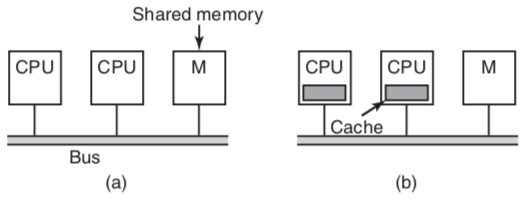
\includegraphics[width=.9\textwidth]{images/uma.png}

				\caption{
					Two Bus-Based \uma Multiprocessor Examples: (a) Without caching. (b) With caching.
				}\par
				\label{fig.uma}
			\end{figure}

			The firsts \uma multiprocessors were bus-based architectures where
			the \cpu wait for the bus channel stays free to perform a memory
			access, as illustrated in Figure \ref{fig.uma}(a).
			When the number of cores scale, the bus traffic begin to be a
			bottleneck of the system.
			To solve this problem, a small but fast memory level, called cache,
			are added to each \cpu, as depicted in Figure \ref{fig.uma}(b).
			The cache allowed readings to be resolved locally, reducing traffic
			to the main memory.

			However, many problems of inconsistency and ordering of operation
			on memory arose with the advent of caches.
			For instance, when a write operation dirties a memory address in
			a particular cache, this change must be notified to all other caches.
			Equally important, it is necessary to ensure a specific order in
			the concurrent operations on a given address through different caches.
			The protocols that guarantee these properties are called cache-coherence protocols.

			\begin{figure}[h]
				\centering
				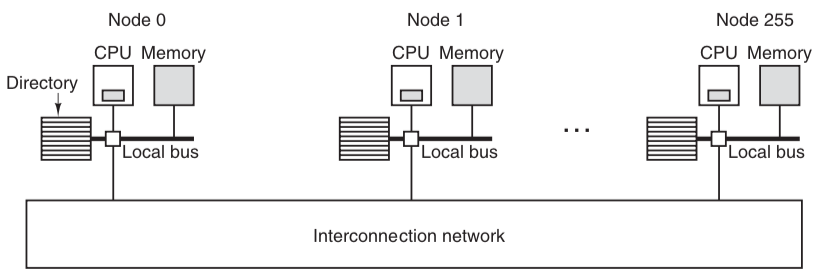
\includegraphics[width=.8\textwidth]{images/numa.png}

				\caption{
					\numa Multiprocessor Example.
				}\par
				\label{fig.numa}
			\end{figure}

			Nevertheless, the numbers of cores in \uma multiprocessors are limited
			to a few dozens of \cpus.
			Thus, to allow hundreds of cores to communicate, \numa machines provide
			a single address space visible to all \cpus through an interconnection
			network,  as illustrated in Figure \ref{fig.numa}.
			Therefore, distributing a virtual memory space among local physics memories,
			the access is guaranteed via load and store instructions.
			Although the time to access to remote memory is slower than to local ones,
			this granted that all \uma programs will be able to run on \numa machines
			but with worse performance.

			\begin{figure}[h]
				\centering
				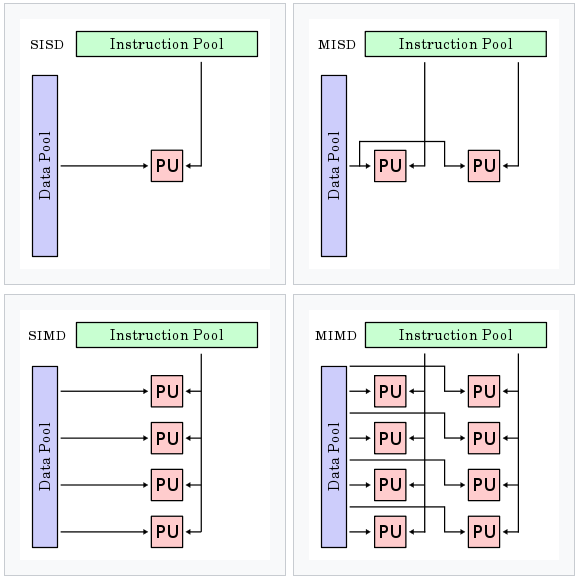
\includegraphics[width=.6\textwidth]{images/flynn.png}

				\caption{
					Flynn's taxonomy:
					(a) \sisd.
					(b) \simd.
					(c) \misd.
					(d) \mimd.
				}\par
				\label{fig.flynn}
			\end{figure}

			In the second place, the workflow classification proposed by Michael J. Flynn~\cite{flynn:1972},
			split multiprocessors architecture based on the number of concurrent
			instruction and data streams available, as depicted in Figure \ref{fig.flynn}.
			First, the most straightforward class, \sisd describes a sequential
			machine which exploits no parallelism in either the instruction or
			data streams, like older uniprocessor machines.
			Second, \simd uses multiple functional units to replicate and operate
			a single instruction over multiples different data streams, like \gpu.
			Third, the most uncommon class, \misd describe multiprocessors that
			apply multiple instructions streams over one data stream.
			Systems that need fault tolerance uses theses multiprocessors, like
			modern flight control systems.
			Finally, a \mimd architecture has multiple processors simultaneously
			executing different instruction on different data, like \xeonphi.

			Currently, two categories of multiprocessors attract attention, the \cmp and \soc.
			\cmps are multicore commercials, which follow a symmetric architecture,
			integrating two or more identical cores into a single die.
			They can have private or shared cache levels, and always share access
			to the RAM.
			Alternatively, \socs are designed with an asymmetric architecture,
			have in addition to the main cores, specialized \cpus in particular
			functions, \eg audio and video encoders, encryption, becoming truly
			complete computer systems on a single chip.

		\subsubsection{Multiprocessor \oses}
		\label{sec.multiprocessor-os}

			\oses are a fundamental part of any computer system.
			They act as an intermediary between users and hardware, with the
			purpose to provide an environment in which users can run programs
			in a conveniently and efficiently manner~\cite{Silberschatz:9ed}.
			Many \os approaches exist in multiprocessor systems.
			In particular, three of them express accurately the difficulties
			of developing \oses targeting the concurrency issues existing in
			such systems.
			Those models are called Replicated, Master-Slave, and Symmetric \os.

			\begin{figure}[h]
				\centering
				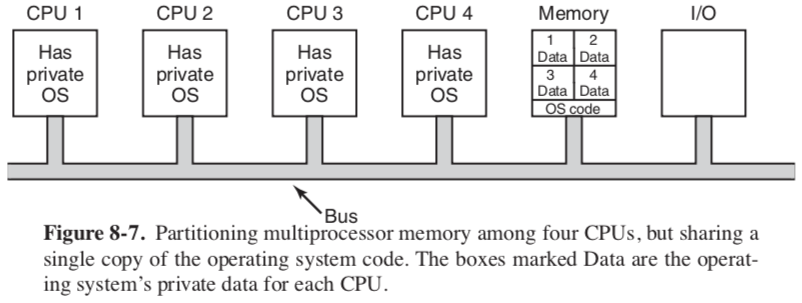
\includegraphics[width=.8\textwidth]{images/replicated-os.png}

				\caption{
					Replicated \os Model.
				}\par
				\label{fig.replicated-os}
			\end{figure}

			The Replicated Model is the simplest way to develop an \os for a
			parallel architecture.
			It only needs to replicate all the internal \os structures for each core.
			Figure \ref{fig.replicated-os} shows how this model allocates fixed memory spaces
			between the cores, giving each of them its private \os.
			The system calls are performed by the calling \cpu, avoiding concurrency issues.
			Also, a producer-consumer model is sufficient for two different \cpus to communicate.

			In the meantime, this model has imperceptible aspects~\cite{tanenbaum:4ed}.
			First, since each \cpu has its own process and page tables, turn impossible
			to optimize the use of resources.
			For instance, if many of processes are waiting for use an overloaded \cpu,
			it is impossible to migrate them to an available \cpu.
			Second, operations with I/O devices can introduce inconsistency problems
			such as the same disk block operated by different \cpus.
			Finally, replication of the internal \os structures makes this model
			impractical for systems with memory constraints.

			\begin{figure}[h]
				\centering
				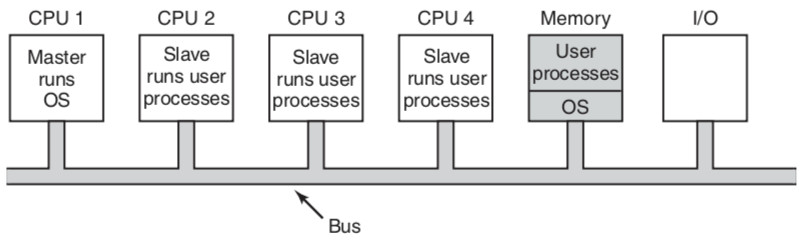
\includegraphics[width=.8\textwidth]{images/master-slave-os.png}

				\caption{
					Master-Slave \os Model.
				}\par
				\label{fig.master-slave-os}
			\end{figure}

			The Master-Slave model began to attract attention with the return of
			processors without cache coherence.
			As Figure \ref{fig.master-slave-os} shows, there is only one copy of
			the internal \os structures, and they all belong to a single \cpu, called master.
			In this way, all system calls performed by a worker \cpu, called slave,
			are redirected to the master.
			With these changes, this model solves the problems of the previous model
			by using only one copy of the data structures.
			For illustration, processes and memory pages can be scheduled and
			distributed dynamically to any \cpus.
			However, when adopting a centralized approach, the master can become
			the bottleneck of the system if it can not handle the number of the
			incoming requisition.

			\begin{figure}[h]
				\centering
				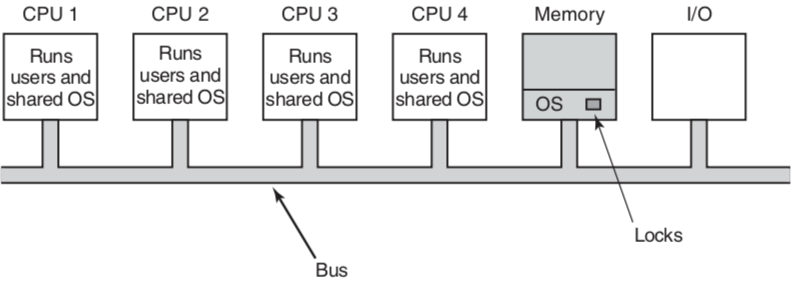
\includegraphics[width=.8\textwidth]{images/smp-os.png}

				\caption{
					Symmetric \os Model.
				}\par
				\label{fig.smp-os}
			\end{figure}

			Finally, the Symmetric model, called \smp, eliminates the centralization
			problem of the foregoing model, as illustrated in Figure \ref{fig.smp-os}.
			So, there is still only one copy of the \os structures but shared in memory.
			When a \cpu makes a system call, it loads the structures and operates on them.
			Consequently, processes and memory pages also continue to be dynamically balanced.
			The difficulties introduced by this model lie in concurrency for \os structures.
			Depending on how the critical regions are managed, the performance of the system
			may be equivalent to the Master-Slave model. So the hardest part is breaking the
			\os into critical regions that will run on different \cpus, where one core does
			not affect the execution of another or fall into a deadlock~\cite{tanenbaum:4ed}.
			Besides, if the hardware does not support cache coherence, the process of
			invalidating the cache may also introduce serious performance problems in \oses of this type.

			As can be noted, the software is always lagging behind the constant hardware advances.
			Many solutions may work very well in specific contexts but should be chosen with care.
			In some cases, in order to extract the maximum performance from a system, it will be
			necessary to redesign the whole process from scratch.

	\subsection{Multicomputers}
	\label{sec.multicomputers}

		Increase the number of cores and still providing a shared memory in a
		single die is very expensive and challenging.
		However, it is more simple and cheap to interconnect more straightforward
		computers in a high-speed network, \eg cluster computing.
		Despite the problem of developing networks and high-speed interfaces
		for communication of the nodes, it is analogous to the problem of
		providing a shared memory in multiprocessors.
		Nevertheless, the expected communication times will be in the
		microseconds, as opposed to nanoseconds of the multiprocessors,
		making things simpler~\cite{tanenbaum:4ed}.

			\subsubsection{Multicomputer Hardware}
			\label{sec.multicomputers-hw}

				A multicomputer node summarizes on an elementary computer, with one or
				more multiprocessors, local \ram and I/O devices.
				In many cases, there is no need for monitors or keyboards, only the
				network interface.
				In this way, it is possible to integrate hundreds or even thousands
				of nodes providing the vision of a single computer.

				\begin{figure}[h]
					\centering
					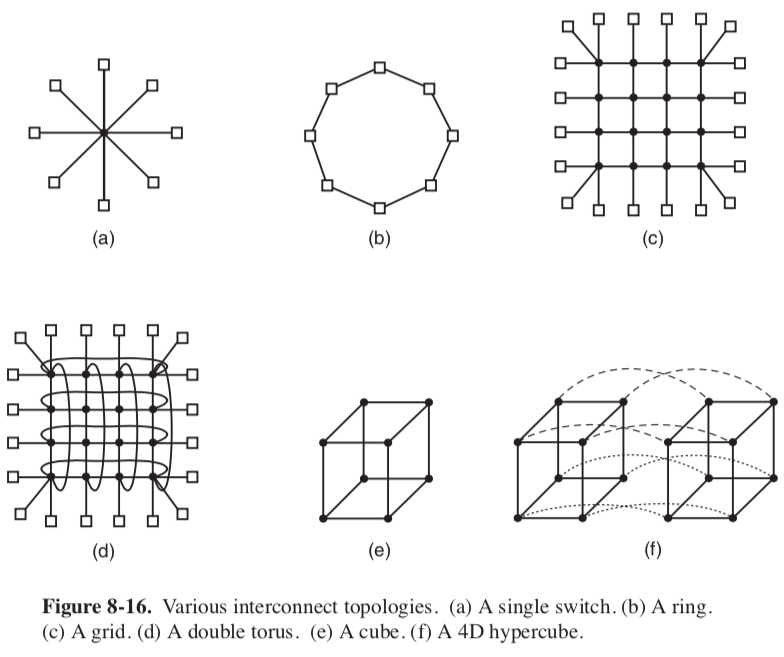
\includegraphics[width=.8\textwidth]{images/net-topologies.png}

					\caption{
						Network Topologies Examples.
					}\par
					\label{fig.net-topologies}
				\end{figure}
				
				A switch set is organized into different topologies to interconnect
				the nodes of a multicomputer.
				As illustrated in Figure \ref{fig.net-topologies}, there are a
				variety of topologies with their own characteristics.
				For instance, commercial multicomputer usually uses bi-dimensional
				topologies such as \textit{grid} or \textit{mesh} because they present
				regular behavior and easily scalable.
				When the goal is to provide higher fault tolerance, in addition to the
				smaller path between two points, the \textit{torus} variant implement
				connections between the extreme points of the \textit{grid}.
				Even multi-dimensional topologies can be used, all depending on the
				characteristics expected from the network.

				There are two types of switching schemes in the multicomputer network.
				The \textit{store-and-forward packet} switching scheme breaks the message
				into fixed-size packets.
				The packets are copied and moved between the switches following a
				routing algorithm until they reach the destination.
				Although flexible and efficient, this scenario can generate a variable
				latency in packet delivery.
				The other scheme, called \textit{circuit switching}, performs a resource
				allocation protocol through all path from source to the destination.
				This protocol ensures a steady communication stream, although the
				slow start and possible sub-utilization of the resources.

			\subsubsection{Low-Level Communication Software}
			\label{sec.multicomputers-low-sw}

				\begin{figure}[h]
					\centering
					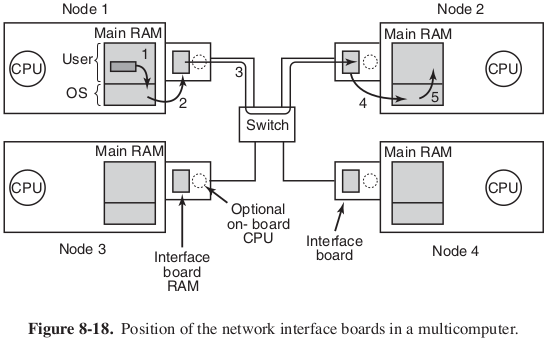
\includegraphics[width=.8\textwidth]{images/multicomputer.png}

					\caption{
						Simple Multicomputer Example.
					}\par
					\label{fig.multicomputer}
				\end{figure}

				Because these boards are built and connected to \cpus and \ram,
				they have substantial impacts on system performance and \os design.
				Virtually, interfaces have enough \ram space to receive/send packets.
				If this address space is actually in main memory, we fall into the same
				problem of multiprocessors in the struggle for the use of the bus channel.
				Thus, in general, network cards have a dedicated memory so as not to
				generate bottlenecks in access to main memory, as illustrated in figure \ref{fig.multicomputer}.

				However, excessive packet copying can degrade the performance of the system.
				Where, in an ideal scenario, four end-to-end copies would be needed,
				\ie from the sender's \ram to the interface memory, from the interface
				to the network, from the network to the memory of the target interface, and,
				finally, to the recipient's \ram.
				Although, depending on how the \os provides access to communication
				resources, that number can grow a lot.
				For instance, mapping the interface into the kernel address space
				rather than the user-space, an extra copy to an internal kernel
				buffer is required.
				Thus, for performance reasons, modern systems already map the interfaces
				to user-space address.
				Nonetheless, they introduce problems of concurrency between the various
				users by the communication resources.

				Processors may also have one or more \cpus specialized in
				communication procedures, called \dma.
				\dmas can make copies between system memories, send/receive packets
				without the main \cpus waste cycles dealing with network interfaces
				or main memory access bottlenecks.
				However, such intermediate copies lead to overhead on system structures,
				such as cache, \tlb, or page management.
				Furthermore, introducing concurrency issues in the interaction between
				\cpus and existing \dma channels.

			\subsubsection{User-Level Communication Software}
			\label{sec.multicomputers-user-sw}

				The low-level mechanisms discussed above allow \cpus on different
				computers to communicate through the messages exchange by
				send/receive primitives.
				The basic configuration needed for send primitive is knowing the
				recipient identifier and the message.
				On another hand, the receive primitive needs to identify which of
				the network interfaces it should configure and where to write the
				incoming data.

				\begin{figure}[h]
					\centering
					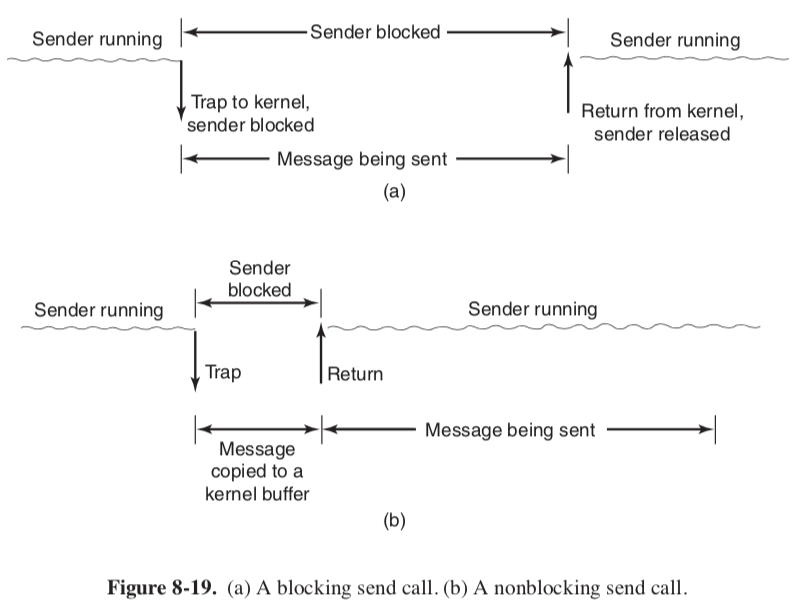
\includegraphics[width=.8\textwidth]{images/calls-types.png}

					\caption{
						Calls Types:
						(a) synchronous call.
						(b) asynchronous call.
					}\par
					\label{fig.calls-types}
				\end{figure}

				There are two approaches to implementing these primitives, either
				through blocking or non-blocking calls, as illustrated in Figure \ref{fig.calls-types}.
				Blocking calls, called synchronous calls, block the requesting \cpu
				until complete the procedure.
				Non-blocking calls, called asynchronous calls, return control to the
				\cpu while the procedure is still in progress.
				Although asynchronous calls provide better performance than
				synchronous ones, they introduce some disadvantages where the sender/receiver
				cannot use the message buffer before the operation is complete.

				According to Tanenbaum, there are four ways to implement send primitive:
				\begin{itemize}
					\item \textbf{Blocking sending:} \cpu hibernates or schedules another
						process, while the message is transmitted.
					\item \textbf{Non-blocking sending with copying:} realizes an extra copy of
						the message to a kernel buffer, degrading performance.
					\item \textbf{Non-blocking sending with interrupt:} notifies the \cpu
						when the send finishes, where the buffer must remain untouchable,
						difficulting the programmability.
					\item \textbf{\cow:} management of buffers to make an extra copy only
						when needed, but can copy unnecessarily.
				\end{itemize}

				Analogous, there are other four forms to implement the receive primitive:
				\begin{itemize}
					\item \textbf{Blocking receive:} \cpu hibernates or schedules another
						process until a message is received.
					\item \textbf{Non-Blocking receive with messages pool:} \cpu creates
						a buffer to store incoming messages, then consumes from it when
						there is some message available, requiring synchronization.
					\item \textbf{Non-Blocking receive with Pop-up Threads:} creates a specific
						thread upon receiving a message to perform the necessary operations.
						But, consumes resource for creating and destroying the thread.
					\item \textbf{Non-Blocking receive with interrupt handlers:} the receiver
						is interrupted to execute a handler when receiving a message.
						Presents a better performance than create a thread but difficult
						the programmability.
				\end{itemize}

				Some of the implementation approaches may be hardware dependent.
				However, choosing the ideal approach is still the responsibility of the \os designer.
				Even so, the distributed nature of multicomputers forces developers to
				use a messaging strategy regardless of what the hardware has to offer.
	
	\section{Kalray MPPA-256 Lightweight Manycore Processor}
	\label{sec.mppa}

		\begin{figure}[h]
			\centering
			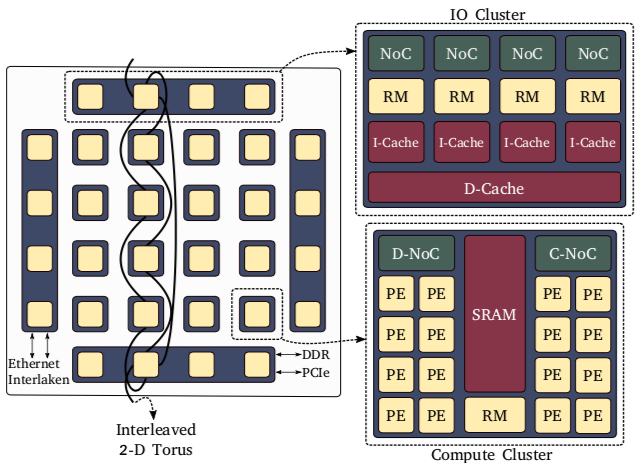
\includegraphics[width=.7\textwidth]{images/arch-mppa.png}

			\caption{
				Architectural overview of the \mppa processor~\cite{Penna2018}.
			}\par
			\label{fig.mppa-arch}
		\end{figure}

		The \mppa is a high-performance, low-power multicore processor
		developed by the French company Kalray.
		Developed to handle \mimd workloads, \mppa mixes features of
		multiprocessors and multicomputers on a single chip.
		Precisely, the multiprocessor model is used inside a cluster
		to coordinate the cores and the local resource balancing, and
		follows a multicomputer model in inter-cluster communication.

		As illustrated by Figure \ref{fig.mppa-arch}, the used version of
		the architecture, called Bostan, has 256 general-purpose cores and
		32 cores for system use, called \pes and \rmans, respectively.
		The processor use 28~mm CMOS technology and all cores run at 500~MHz.
		Besides, all cores have caches and \mmus with software-managed \tlbs.
		Finally, the 288 cores are grouped into 16 \cclusters, dedicated to
		the payload, and 4 \ioclusters, responsible for communicating with peripherals.

		Each \ccluster features 16 \pes, an \rman, an \noc interface and 2~MB of \sram.
		The hardware does not support cache coherence to improve energy consumption.
		On the other hand, \ioclusters have only 4 \rmans with cache coherence support,
		4 \noc interfaces, and 4~MB of local \sram added to 4~GB of \dram.

		The address space on each cluster is private, forcing exchange messages
		by one of two different interleaved 2-D Torus \nocs.
		On the one hand, the \cnoc is exclusive to 64-bit control messages,
		usually used for synchronization.
		On the other hand, intense exchange data occurs through the \dnoc.
		Additionally, all clusters have available \dmas associated with each
		\noc interfaces to handle communication issues.

		As discussed in Section \ref{sec.multicomputers-user-sw}, the \noc interfaces
		expose communication resource to perform send and receive primitives
		like network interfaces.
		Accurately, they summarize the following resources:

		\begin{itemize}
			\item 128 slots for receiving commands;
			\item 256 slots for receiving data;
			\item 4 channels for sending commands;
			\item 8 channels for sending data, and;
			\item 8 $\mu$threads for sending asynchronous data
				(They need to be associated with a transfer channel).
		\end{itemize}

		The configuration of these features is accomplished by a mix between
		writing on \dma registers and performing syscalls to a hypervisor
		that virtualizes the \mppa hardware.	
	
\section{Hardware Abstract Layer for Lightweight Manycores}
\label{sec.hal}

	\begin{figure}[h]
		\centering
		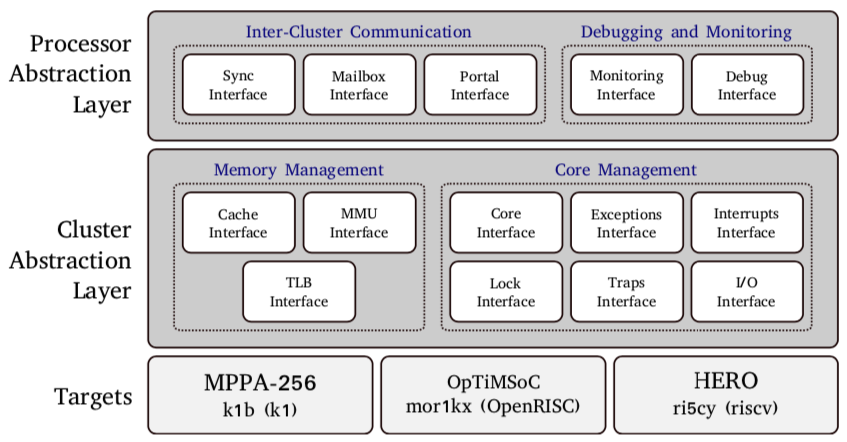
\includegraphics[width=.9\textwidth]{images/hal-struct.png}

		\caption{
			Structural overview of the proposed \hal~\cite{penna:compas2019}.
		}\par
		\label{fig.hal-struct}
	\end{figure}
	
	Despite the benefits of scalability and energy efficiency gained with the
	emergence of the \textit{lightweight \manycores}, they sin in programmability
	and portability.
	Several current research is focusing on the challenges that have arisen with
	these processors~\cite{christgau2017, gamell2012, serres2011}.
	For instance, the study and development of full \oses running on them.
	However, Pedro H. Penna \etal believe that significant barriers will still
	arise in this scenario, and the solution is to rethink \os design from scratch.
	For this, we propose a generic and flexible \hal around the intrinsic
	architectural characteristics of the \textit{lightweight \manycores}.
	Currently, \hal is being developed for \mppa~\cite{DeDinechin2013-1} and
	\optimsoc~\cite{Wallentowitz2013}.

	Unlike other research that aims to design a fully-featured \os~\cite{Baumann2009,kluge2014,nightingale2009,rhoden2011},
	the \hal belongs in one level below.
	It is the first layer on top of the hardware and should provide a standard
	view of these emerging processors for a client applications, \eg \os.
	As illustrated in Figure \ref{fig.hal-struct}, this \hal is structured in
	two major logic layers: \textit{Cluster Abstraction Layer} and \textit{Processor Abstraction Layer}.

	The \textit{Cluster Abstraction Layer} encapsulates the management of a single cluster.
	It provides two modules, \textit{Core Management}, and \textit{Memory Management}.
	The \textit{Core Management Module} aims to provide to a client application a complete
	thread synchronization and management system, rich support of handling
	interrupts/exceptions, and an adequate system call interface.
	The \textit{Memory Management Module} provides a uniform view of the \tlbs
	and paging systems with maintenance routines for them and the cache.
	Therefore, some design decisions are made to create interfaces that are not
	dependent on the underlying hardware.
	For example, a context switch mechanism was not provided in the
	Core Management module because this would force the client \os
	to write code in assembly, hurting the conceptual idea of the \hal.

	The \textit{Processor Abstraction Layer}, in particular, embraces
	architectural features related to multiple clusters.
	The \textit{Inter-Cluster Communication Module}, the focus of
	this monograph, exports three main abstractions to allow the
	cluster to exchange data between them, based on ideas proposed along with the
	\nodeos distributed runtime system~\cite{DeDinechin2013-1}.
	These abstractions will be presented in Section \ref{sec.inter-cluster-communication}.
	Lastly, the \textit{Monitoring and Debugging Module}, as the
	name shows, exports routines to aid debugging and extraction
	of diagnostics about hardware metrics, such as the number of
	page-fault or detour taken.

\section{Inter-Cluster Communication Module}
\label{sec.inter-cluster-communication}

	The following sections conceptually present the three abstractions
	that will be proposed for \hal and implemented over \mppa.
	They are the \sync, \mailbox, and \portal abstraction.
	The purpose of developing more specific abstractions than
	send and receive primitives, described in Section \ref{sec.multicomputers-user-sw},
	is to provide more precise and easy-to-use mechanisms for
	\os and client applications.
	On top of them, it is possible to create all kinds of essential
	services such as message passing and synchronization,
	to more elaborate services such as shared memory regions~\cite{penna:rmen}.

	A related point to consider is that mechanisms described below refer
	to interactions between distinct clusters only.
	The implementation can follow synchronously or asynchronously models,
	as described in Section \ref{sec.multicomputers}, depending only on hardware support.
	In the same way, it is worth be noted that the small messaging exchange
	is decoupled from abstraction to intense data transfer.
	The motivation for this, as other details, is to exhibit better control
	over the \qos to the higher layers.
	For instance, the use of distinct \nocs for each service.

		\subsection{Sync Abstraction}
		\label{sec.sync-abs}

			\begin{figure}[h]
				\centering
				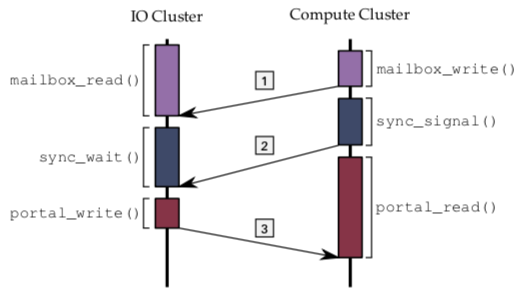
\includegraphics[width=.7\textwidth]{images/conceptual-sync.png}

				\caption{
					Synchronization Abstraction Concept.
				}\par
				\label{fig.conpt_sync}
			\end{figure}

			The \textit{Synchronization Abstraction}, called \sync, proves bare bones
			for cluster synchronization.
			It enables a set of clusters to wait for a notification coming from a
			specific cluster.
			The behavior is analogous to the \posix signal abstraction, but the \sync
			provides only the case of notification.
			Specifically, as can be seen in Figure \ref{fig.conpt_sync}, the
			cardinality of the operation is N:1, where N clusters wait for 1 Cluster
			to send a notification.

		\subsection{Mailbox Abstraction}
		\label{sec.mailbox-abs}

			\begin{figure}[h]
				\centering
				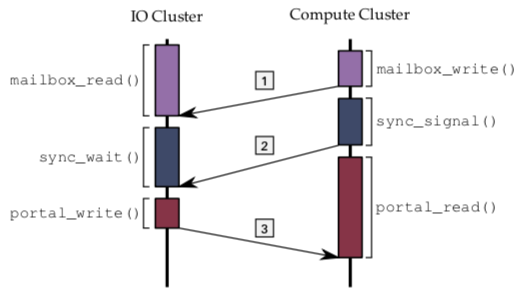
\includegraphics[width=.7\textwidth]{images/conceptual-sync.png}

				\caption{
					Mailbox Abstraction Concept.
				}\par
				\label{fig.conpt_mailbox}
			\end{figure}

			The \textit{Mailbox Abstraction} allows clusters to exchange fixed-size
			messages with each other.
			The message was thought to be a relatively small size, usually a few hundred bytes.
			Similarly, the operation of the \mailbox follows \posix message queue behavior.
			For example, the message can be used to encode small operations and system
			control signals.
			As illustrated in Figure \ref{fig.conpt_mailbox}, the cardinality of the operation
			is N:1, where N senders can send messages to 1 receiver queue.

		\subsection{Portal Abstraction}
		\label{sec.portal-abs}

			\begin{figure}[h]
				\centering
				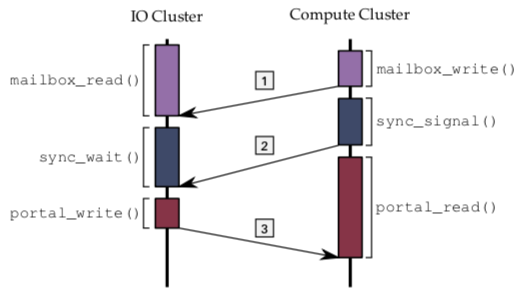
\includegraphics[width=.7\textwidth]{images/conceptual-sync.png}

				\caption{
					Portal Abstraction Concept.
				}\par
				\label{fig.conpt_portal}
			\end{figure}

			Lastly, the \textit{Portal Abstraction} enables two clusters to exchange arbitrary
			amounts of data.
			The conceptual idea of ​​the \portal is similar to that implemented in \posix pipes.
			Figure \ref{fig.conpt_portal} shows the \portal operation, with cardinality
			1:1, a cluster pair opens a channel to transfer data.
			However, the operation is only allowed in one sense, that is, one
			cluster must assume the role of the sender and the other of the receiver.
